\chapter{Science Is Elementary 3}

% \begin{figure}[H]
%     \centering
%     \includegraphics[width=\textwidth/2]{./Games/EveryChildCanSucceed/Images/EveryChildCanSucceed7CD.png}
%     \caption{Every Child Can Succeed 7 CD}
% \end{figure}

The final of the Science Is Elementary games published and released by The Lightspan Partnership for the PlayStation 1.

Science Is Elementary 3 features three video programs:

\begin{itemize}
    \item Let's Explore Air
    \item Let's Explore Weather and the Seasons
    \item Let's Explore Soil and Rocks
\end{itemize}

\clearpage
\newpage

\section{Let's Explore Air}

\subsection{Audio Summary}

In "Let's Explore Air", we investigate where air exists, and discover what wind is. We emphasise the importance of clean air to all living things. In the exploration, we ask 'what is inside an empty jar?'

\subsection{Transcription}

Young Girl: What's inside of these bubbles? What's around them? Where can you find air around you? Wind is air that's moving. What can wind do? Most of the time you can't see air, so how do you know it's there? How do all living things use air? What are some ways people use air? Watch this story and see if you can tell me, 'Where is Air?'

Narrator: Where is air? Is it right up there? Is it down below? Is it everywhere you go? Where is air? Is it where you sleep? Is it where you play? Is it with you night and day? Where is air? Is it with birds and these walruses and fleas, flowers and trees? Where is air? It's everywhere!

Young Girl: What do these children and their teacher discover about air?

Teacher: Guys, here is a glass, okay, and what I'm going to do is, this is just a regular piece of tissue paper. Now I'm going to put the tissue paper in the glass, and I want to know what do you think is going to happen if we put that glass with the tissue paper in it, in the water? What do you think will happen to the piece of paper? Chris.

Boy 1: I think the tissue paper is going to get wet.

Teacher: The tissue paper's gonna get wet? What do you think, Jonathan?

Boy 2: Same thing.

Teacher: Yeah, you think so? Yeah. Mariella?

Girl 1: The tissue paper is going to get wet.

Teacher: Okay. How about you, Jed?

Boy 3: I think the tissue paper will stay in the glass and get wet.

Teacher: You think it's going to stay in the glass but it's gonna get wet? Alright.

Girl 2: I think the paper is going to stay in, but the air that's in the tank is gonna keep the paper dry.

Teacher: Okay. Who would like to try to put the glass in upside down in the water? Hold it there. Let's pull it out and see what happens to it.

Girl 1: Woah, it's dry!

Teacher: What happened to the glass? Why do you think it's dry? What do you guys think about this, now that it is dry? You want to touch it? Go ahead, touch it. Why didn't the tissue get wet, Mariella?

Girl 1: Because the air didn't let the water go in the glass.

Teacher: Where is the air?

Girl 1: Under the tank.

Teacher: Under the tank, and where else do you think it was? If it didn't let water go into it, where else was it? Jonathan, where else was the air.

Boy 2: It was in the glass.

Teacher: It was in the glass, yeah, you're right. And that's what [Robo] at first predicted.

Girl 2: I said that the tissue paper is gonna stay in the glass, and the tissue paper was not gonna get wet.

Teacher: Right. And why isn't the tissue paper wet now, now that we know what Mariella said?

Girl 2: Because the air didn't let the water go in the glass.

Teacher: Great. The air didn't let the water into the glass. Was the glass empty?

Girl 1: No.

Teacher: What was in it then?

Girl 1: Air.

Teacher: Air, yeah. Air. So is air nothing or is it something?

Children together: It's something.

Teacher: Yeah, it takes up space. And it took up space of a\dots

Chidren: Glass.

Teacher: Glass.

Boy 3: What would happen if we put the glass in at an angle?

Teacher: Okay, well let's see and try to find out. Here we have the paper in the glass. Why don't you try to do it [Jed]? What were those bubbles [Jed]?

Boy 3: Air.

Teacher: Yeah, they were air. When the bubbles came up, what was happening to the glass? What was going in the glass?"

Girl 2: Water.

Teacher: And what happened to the paper?

Girl 2: It got wet.

Teacher: Got wet, yeah. As the air left, the water went into the glass. Good job.

Young Girl: How does this wind chime work? How can you make a wind chime that works for you? Well, it's really easy. The first thing to do is to get a board, spoons, and strings. Then you put the board somewhere where it's really nice and windy. Then what you do is that you tie the strings around the board and then you let them hang. Then you take the spoons and then you tie them around, so the spoons can make the music for you, like this. And then your wind chime works. You try it.

\subsection{Credits}

Executive Producer/Director Writer: Larry Walcoff;
Editor/Camera: Nick Kolias;
Host: Francesca Pellerano;
"Air" Teacher: Jackie Benchik;
Feather Puppet: Marilyn Price;
Production Coordinator: Nancy Schlafer;
Instructional Designer: Dolores J. Deardorff, Ed.D.;
Science Consultants: Denise E. Lessow, Ed.D., Eric Worch, Indiana University School of Education;
Content specialists: Bob McDonald (Toronto, Canada);
Post Production Facility: Corplex, Inc.;
AIT Executive Producer: Frank Batavick;

\section{Let's Explore Weather and the Seasons}

\subsection{Audio Summary}

In "Let's Explore Weather and the Seasons", we consider different kinds of weather and how it changes through the seasons. How weather and seasons affect us is illustrated. The exploration section looks at how a school building protests students from seasonal weather.

\subsection{Transcription}

Young Girl: No question about it, it can be cold out when it's Winter in my city. How do you like my outfit? How do you dress for the weather?

Boy 1: I think this is Winter.

Girl 1: And why do you think this is Winter?

Boy 1: Well, because it has white snow and it looks very cold.

Girl 1: Mmm hmm.

Boy 1: What season do you think this is?

Girl 1: I think this is Spring.

Boy 1: Why do you think it's Spring?

Girl 1: Because it looks warm out there are lots of flowers.

Boy 1: What season do you think this is?

Girl 1: I think this is Summer because it looks like it's at the beach and usually people only go to the beach when it's Summer. What season do you think this is?

Boy 1: I think it's Fall because all the leaves are red, brown in different colors.

Young Girl: What is it that determines how we dress? Each season is different. How do you play in each season? Guess why they call this season Fall? The leaves Fall to the ground. In Winter, the tree looks dead. Is it? In the Spring what happens to the tree? And in the Summer the leaves look like this. And then it's Fall again. A year's past, hasn't it? Most places on Earth have four seasons. What do you see around me that shows you what season it is? What do you see that shows you what season it is?

"Summer Is..." This story, written by Charlotte Zolotow with pictures by Janet Archer, tells us how some children feel about different times of the year.

Summer is birds singing. Summer is bare feet and daisies and dandelions and roses full on their stems. Summer is porches and cold lemonade and dogs sleeping in the shade.

Fall is squirrels on rooftops. Fall is red and yellow leaves and trees bending in the wind. Fall is people holding their hats. Fall is chrysanthemums and dry leaves and pumpkins and cider and honey and baskets of apples on the roadside stands.

The Winter is waking to the scrape of shovels. Winter is snow suits and heavy underwear. Winter is sleds and ice skates and the wind. Winter is snow and pink skies early in the evening. Winter is a white sun and the moon before you're tired.

Spring is pussy willows and yellow crocus pushing through the melting snow. Spring is a smell of wet earth and growing things. Spring is the world waking once again.

"Summer Is..." by Charlotte Zolotow is available in most school and public libraries.

What do these children and their school teacher discover about their school building and how it protects them from changes in the weather?

Teacher: What a messy day it is outside today. What's happening? Who knows? Beth, do you know?

Beth: It's a very snowy and slushy day.

Teacher: It certainly is. What is the temperature this morning, Victor?

Victor: About 32 degrees from outside.

Teacher: Mmm hmm. What's the temperature inside?

Girl 2: About 72 degrees.

Teacher: Mmm hmm. It's colder outside than inside, isn't it? Why is there a difference in temperature? What is making it warmer inside?

Girl 3: Cus inside they had the heater.

Teacher: Ahmed, can you feel any air coming up from the heater?

Ahmed: Yes.

Teacher: What kind of air is it?

Ahmed: Hot, hot air.

Teacher: Hot air. So it's keeping us nice and warm inside here. What else in this room protects us from the weather outside? Alexandra?

Alexandra: These windows protect us from the outside.

Teacher: How do these windows protect us?

Beth: It protects us because there's two pieces of glass, one on the outside, one on the inside.

Teacher: Very good. Why do we have two sets of doors out here?

(new scene)

Teacher: We have a set here and a set over here. Beth?

Beth: So that when this door opens, the wind and the cold comes in here, but this door closes before that door can open.

Teacher: Very good, Beth.

(new scene)

Teacher: How do roofs on buildings protect us? Timothy?

Timothy: When it's raining outside, the roof will keep us dry.

Teacher: Very good. Christina?

Christina: It keeps the sun off of us on hot days.

Teacher: Very good. Alexandra?

Alexandra: It keeps the snow off of us too.

Teacher: Eric?

Eric: It keeps us warm from the wind. It protects us.

Teacher: Very good.

Ahmed: And you know what?

Children togetehr: What?

Ahmed: The whole building protects us from the weather.

Teacher: Very good.

Young Girl: Would you believe that today's weather makes me feel happy? Most people don't like the rain, but I love it. And I'm drawing a picture to show how I feel. Look out of your window and draw a picture about how the weather makes you feel. Show the picture to a friend and talk about it. You try it.

\subsection{Credits}

Executive Producer/Director Writer: Larry Walcoff;
Editor/Camera: Nick Kolias;
Host: Francesca Pellerano;
"Weather" Teacher: Jolene Nakayama;
Special Thanks: The Sacred Heart Schools, Sheridan Road, Chicago;
Summer Is... Author: Charlotte Zolotow;
Watercolor Pictures: Janet Archer;
Production Coordinator: Nancy Schlafer;
Instructional Designer: Dolores J. Deardorff, Ed.D.;
Science Consultants: Denise E. Lessow, Ed.D., Eric Worch, Indiana University School of Education;
Content specialists: Bob McDonald (Toronto, Canada);
Post Production Facility: Corplex, Inc.;
AIT Executive Producer: Frank Batavick;

\section{Let's Explore Soil and Rocks}

\subsection{Audio Summary}

In "Let's Explore Soil and Rocks", we define rock, soil and sand, and examine their uses. We also discover the importance of these materials to farming. The exploration investigates what rock, soil and sand are made of.

\subsection{Transcription}

Young Girl: Take a closer look. What is this stuff made of?

Boy 1: Soil is made out of worms.

Girl 1: Soil is made out of dirt.

Girl 2: The ground is made of rock and sand.

Girl 3: There's bugs in the soil.

Boy 2: *shrugs*

Girl 4: Soil is sometimes wet.

Boy 3: Soil is black.

Boy 1: And probably\dots

Girl 5: You know what, soil [comes in] rock and sand.

Boy 4: And there's dead stuff in soil.

Boy 1: Dead kind of animals and, uh\dots Gotta look in the encyclopedia.

Boy 5: Soil's made out of rocks, falling leaves, dirt and sand.

Young Girl (voice over): Watch to see what this teacher and some students discover about soil in rocks.

Teacher: What do you see in this pot?

New Girl 1: Dead leaves.

Teacher: Okay, you see some leaves, right? That's part of soil, but what's this stuff?

Children Together: Dirt and water.

Teacher: Yes, some dirt and water. Yes, excellent. I'm going to give you some of it to look at. Just feel it. Use all of your senses when you're looking at dirt and when you're feeling dirt and when you're smelling dirt. You can use your magnifying glass again if you like. Use your nose to smell it with. Use your fingers to feel it. Use your eyes to see it. I don't know if you want to taste it or not. Probably not. But go ahead and feel it and look at it. What do you notice?

New Girl 2: Bits of bark.

Teacher: Okay, very good. What else?

New Child (unknown): Leaves, dead leaves.

Teacher: Dead leaves, worms, rocks, bark. What is it?

New Girl 1: Sand.

Teacher: There's some sand in this soil too. Healthy soil has sand in it. Little bits of that rock get in the soil and that's part of the soil or the dirt. Very good. What we're going to look at next is another kind of material. What is this?

New Girl 1: Sand.

Teacher: This is sand. Yes. Let's look, look at this.

New Girl 3: And Water.

Teacher: Oh, you've noticed something already about this sand.

New Girl (unknown): It's moist.

Teacher: What makes it moist?

New Girl (unknown): Water.

Teacher: There's a little bit of water in this sand. Now take your magnifying glass and look real closely at this sand.

New Girl 1: It has little chips in it.

Teacher: Chips of rock in it. Very good. Okay, anything else?

New Girl 1: It has different colors.

Teacher: Different colors, again. Okay, very good. So now what do we know about sand?

New Girl 2: It's color.

Teacher: It's color.

New Girl 2: It's gypsum rock.

Teacher: It's gypsum rock, little pieces of rock. Okay, does it stick together? Uh-huh. And what's making it stick together?

Children Together: Water.

Teacher: Water. The water in it is making it stick together. Very good. Can you get something off of your rock?

New Girl 1: On the bottom.

Teacher: On the bottom. Okay, you're wiping things off. And if you took a piece of rock and you rubbed it against your big rock, I bet you would see something too [inaudible]. Okay, let's put our rocks down now and just see what kinds of things, little specks of things have come off of this rock. What do you notice? Anything at all? Look through your magnifying glass and see. What do you see? Look, look closer and see what else.

New Girl 1: Sand.

Teacher: Andrea's saying that she sees sand. Do you see any sand?

New Girl 2: Yeah.

Teacher: Yeah. You're getting sand off of your rock. Okay, let me have these little rocks again here. Thank you. So let's think about what we just, what we just found out. What do you suppose a rock is made out of?

New Girl 1: Dirt.

Teacher: We got dirt. What else?

New Girl 2: Sand.

Teacher: Sand. Okay, so when we see things like dirt and sand, we know that there are little bits of rock in that, right? Because that's what, that's how you got the sand. Okay, excellent.

Young Girl (voice over): Sand is rock that has been worn down. Soil is wet sand with other stuff in it. So most rocks are made up of the same stuff: sand and soil. What do you see happening to change the rocks? What's rubbing against the rocks to make the soil? See, wind and water and even roots of plants can slowly change rocks into sand and soil. This is Ashley. See if you can discover what's so special about the soil on her farm.

Ashley: This is my farm. I live here. The reason I live here is because of this good soil which has a lot of organic stuff which makes it good for the plants to grow in. Each year in the Spring, we get out the tractors and we plant seeds in the ground. We hope it rains, but not too much. Each Fall we pick the crops for you and me to eat. Our corn grows well here because of our good soil. It is even good to eat. Not just people like corn, but animals like it too. This part of the farm we don't grow anything because it is very sandy and hardly has any nutrients or good stuff for the plants to grow in, but it is fun to play in. We don't farm in this part of the farm either because it has a lot of rocks and the rocks get in the way of the tractors and seeds won't grow around them.

Young Girl: This wall is very pretty. How else do people use rocks and soil?

Young Girl (voice over): How can people make beautiful things using rocks, sand and soil?

Young Girl: Find out how many rocks you could find in your neighborhood and bring your most funniest, your most unusual, your strangest rocks to school and compare them with your friend's collection of rocks. You try it.

\subsection{Credits}

Executive Producer/Director Writer: Larry Walcoff;
Editor/Camera: Nick Kolias;
Host: Francesca Pellerano;
"Soil" Teacher: Bonnie Burchfield;
Production Coordinator: Nancy Schlafer;
Instructional Designer: Dolores J. Deardorff, Ed.D.;
Science Consultants: Denise E. Lessow, Ed.D., Eric Worch, Indiana University School of Education;
Content specialists: Bob McDonald (Toronto, Canada);
Post Production Facility: Corplex, Inc.;
AIT Executive Producer: Frank Batavick;

\clearpage
\newpage

\section{Screenshots}

\begin{figure}[H]
    \centering
    \begin{subfigure}{0.45\textwidth}
        \centering
        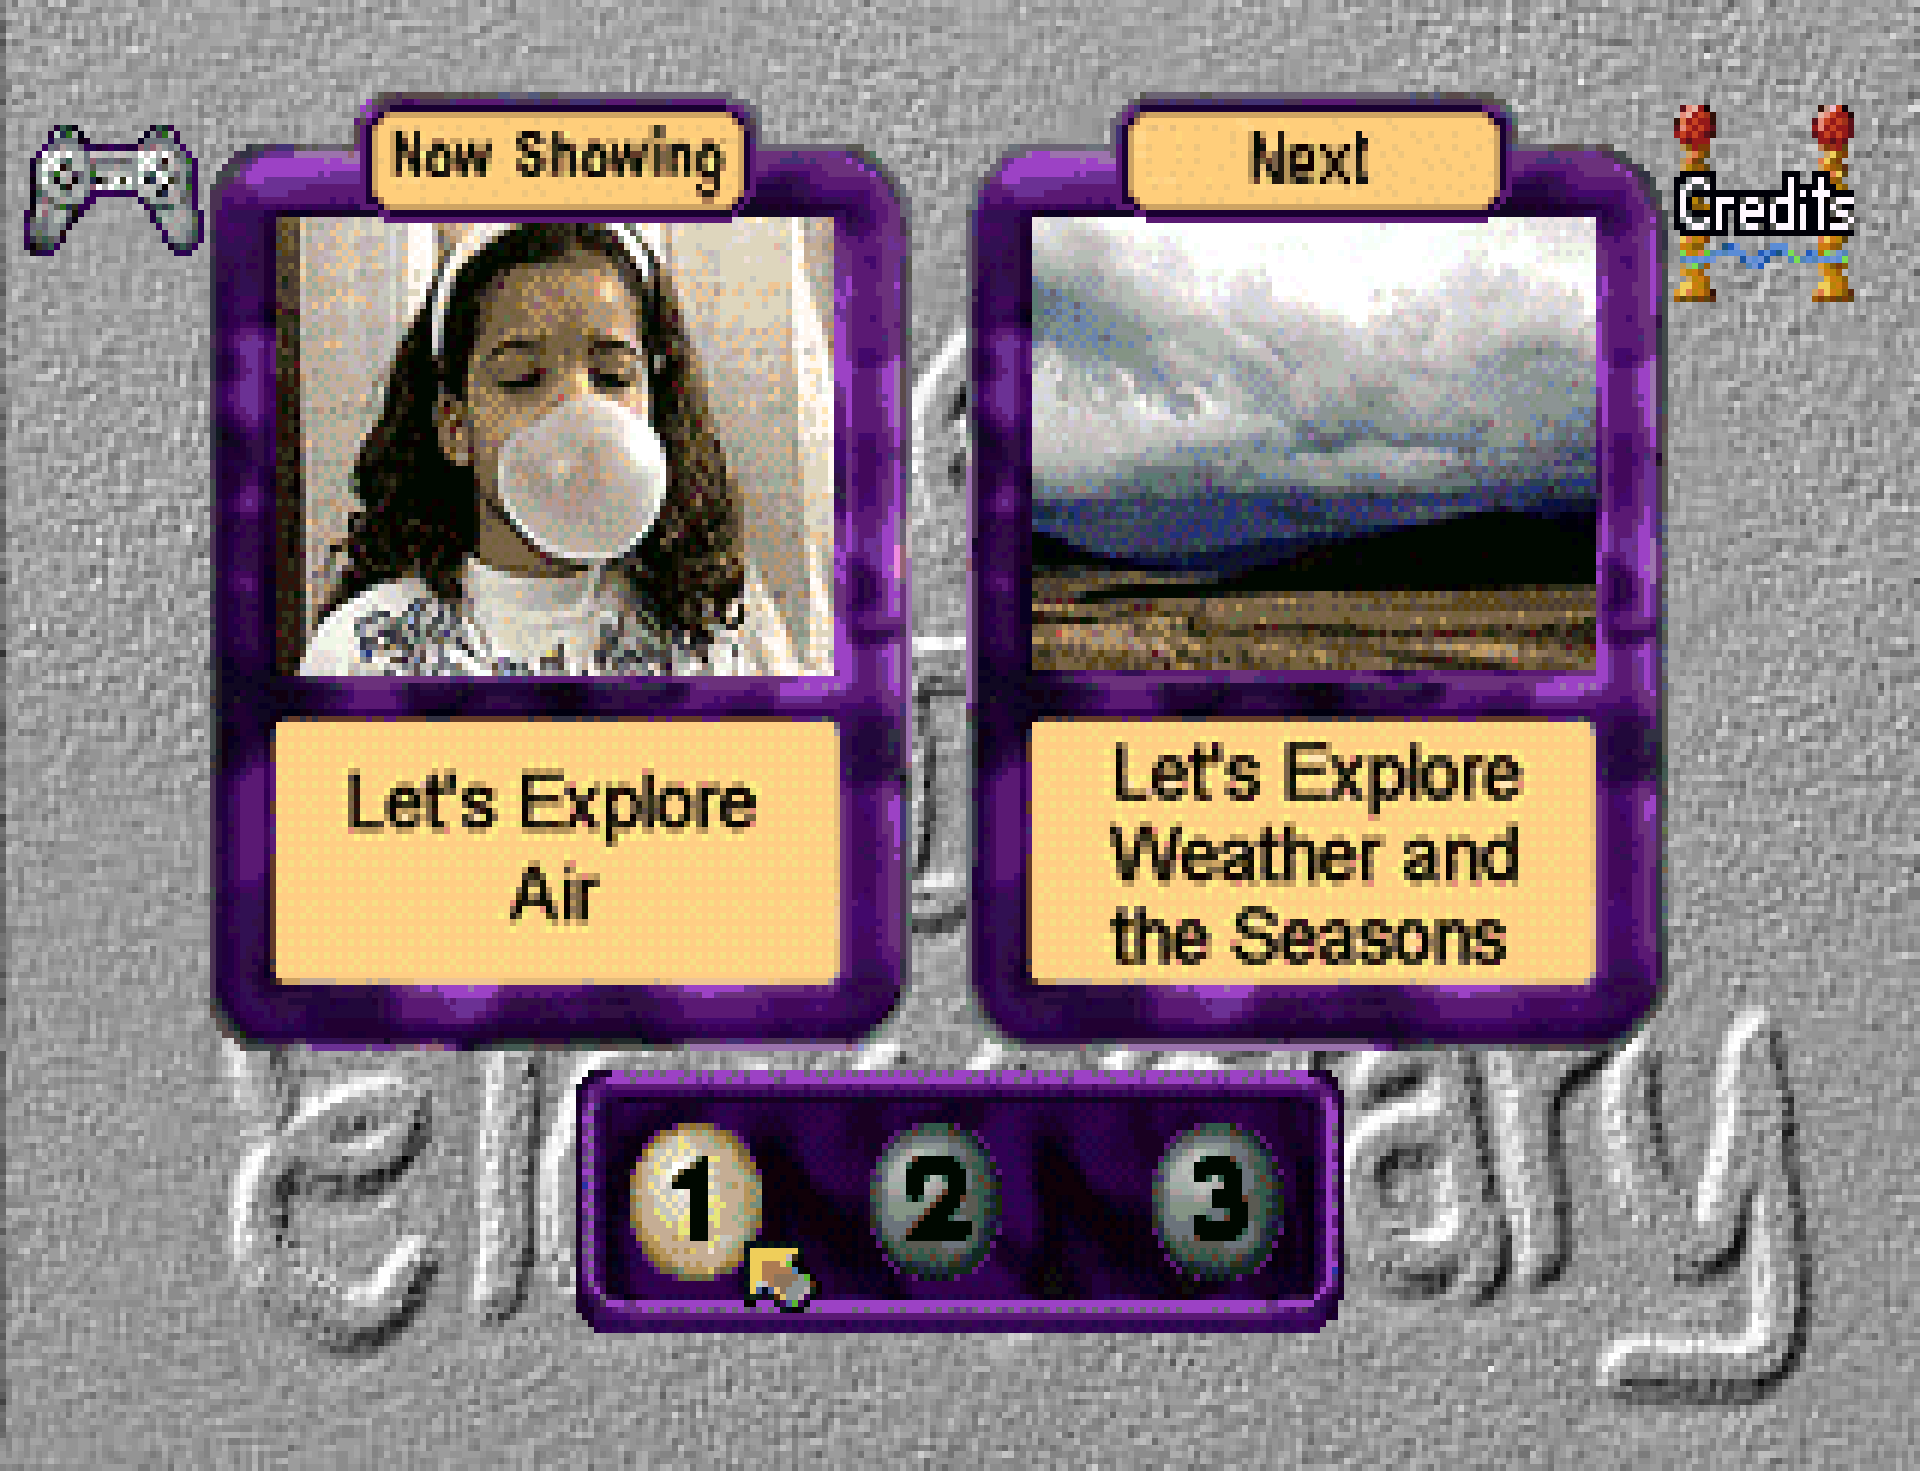
\includegraphics[width=\linewidth]{Games/ScienceIsElementary/Images/ScienceIsElementary3Image1.png}
        \caption{Science Is Elementary 3 - Screenshot 1}
    \end{subfigure}
    \begin{subfigure}{0.45\textwidth}
        \centering
        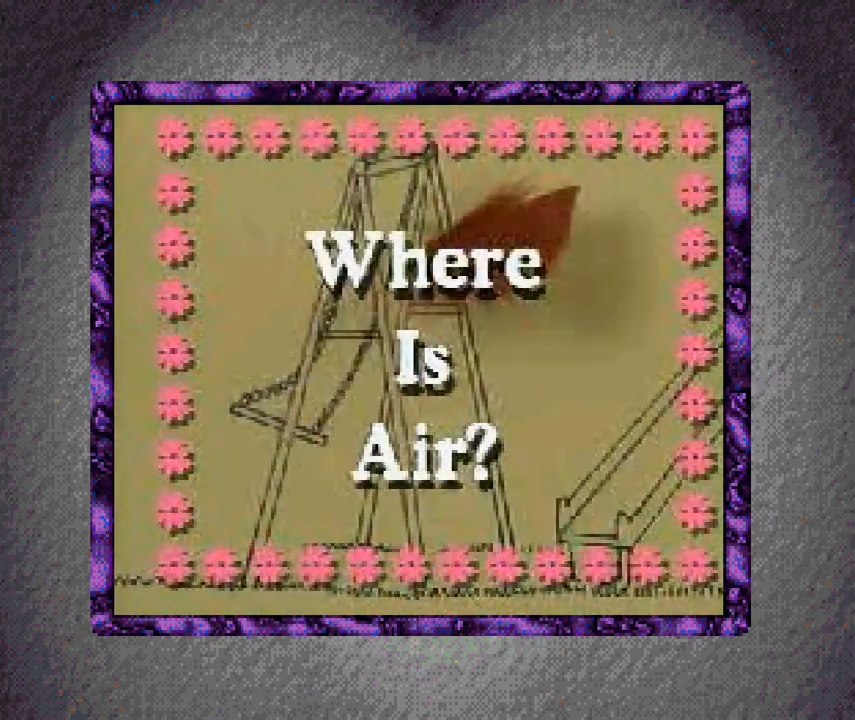
\includegraphics[width=\linewidth]{Games/ScienceIsElementary/Images/ScienceIsElementary3Image2.png}
        \caption{Science Is Elementary 3 - Screenshot 2}
    \end{subfigure}

    \begin{subfigure}{0.45\textwidth}
        \centering
        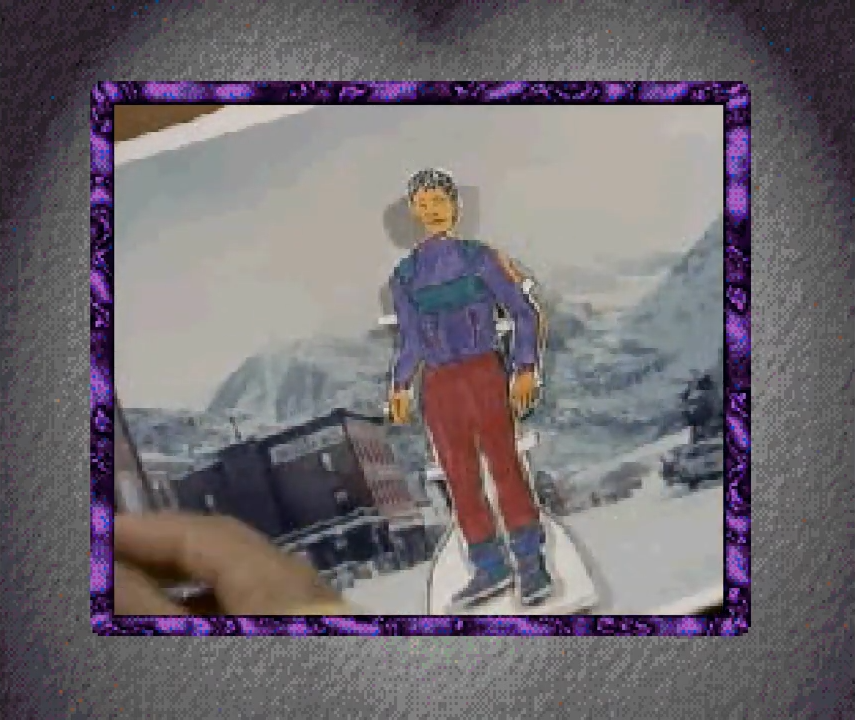
\includegraphics[width=\linewidth]{Games/ScienceIsElementary/Images/ScienceIsElementary3Image3.png}
        \caption{Science Is Elementary 3 - Screenshot 3}
    \end{subfigure}
    \begin{subfigure}{0.45\textwidth}
        \centering
        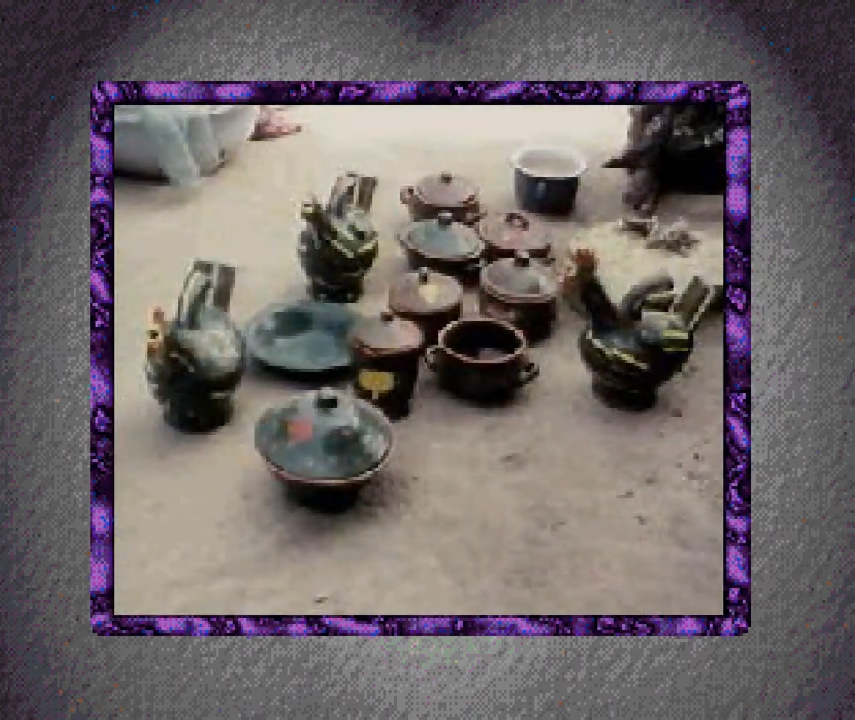
\includegraphics[width=\linewidth]{Games/ScienceIsElementary/Images/ScienceIsElementary3Image4.png}
        \caption{Science Is Elementary 3 - Screenshot 4}
    \end{subfigure}
    \caption{Screenshots from Science Is Elementary 3}
\end{figure}